\documentclass[oneside,fleqn,11pt]{book}
\usepackage[a4paper, total={7.2in, 10.5in}]{geometry}

\usepackage{tikz}
\usetikzlibrary{calc}
\usepackage{setspace}
\usepackage{graphicx}
\usepackage{amsmath}
\usepackage{amssymb}

\DeclareMathOperator\dx{\mathrm{d}\mathit{x}}
\DeclareMathOperator\dy{\mathrm{d}\mathit{y}}
\DeclareMathOperator\dt{\mathrm{d}\mathit{t}}
\DeclareMathOperator\dtheta{\mathrm{d}\mathit{\theta}}
\DeclareMathOperator\cis{cis}
\DeclareMathOperator\sech{sech}
\DeclareMathOperator\csch{csch}
\DeclareMathOperator\cosec{cosec}
\DeclareMathOperator\arsinh{arsinh}
\DeclareMathOperator\arcosh{arcosh}
\DeclareMathOperator\artanh{artanh}
\DeclareMathOperator\Nset{\mathbb{N}}
\DeclareMathOperator\Zset{\mathbb{Z}}
\DeclareMathOperator\Qset{\mathbb{Q}}
\DeclareMathOperator\Rset{\mathbb{R}}
\DeclareMathOperator\Iset{\mathbb{I}}
\DeclareMathOperator\Cset{\mathbb{C}}
\DeclareMathOperator\UQ{Q_3}
\DeclareMathOperator\LQ{Q_1}
\DeclareMathOperator\Med{Q_2}

\usepackage{pgfplots}
\graphicspath{ {./images/} }
\usepackage{bookmark}
\setcounter{tocdepth}{0}
\usepackage{import}
\usepackage{mathtools}

\makeatletter
\g@addto@macro\bfseries{\boldmath}
\makeatother

\DeclarePairedDelimiter{\ceil}{\lceil}{\rceil}
\hypersetup{
	colorlinks   = true, %Colours links instead of ugly boxes
	urlcolor     = blue, %Colour for external hyperlinks
	linkcolor    = black, %Colour of internal links
	citecolor   = red %Colour of citations
}

\newcommand{\tikzAngleOfLine}{\tikz@AngleOfLine}
\def\tikz@AngleOfLine(#1)(#2)#3{%
	\pgfmathanglebetweenpoints{%
		\pgfpointanchor{#1}{center}}{%
		\pgfpointanchor{#2}{center}}
	\pgfmathsetmacro{#3}{\pgfmathresult}%
}

% math font
\usepackage{amsmath}
\usepackage{amssymb}
\usepackage{amsthm}
\usepackage{mathtools}
%\usepackage{arev}

% color
\usepackage[table]{xcolor}

\usepackage[many]{tcolorbox}
\usepackage{pifont}
\usepackage{hyperref}
\usepackage{blindtext}
\counterwithin*{chapter}{part}
\newcommand*{\Part}[2][\partheading]{%
  \refstepcounter{part}%
  \def\partheading{#2}%
  \part*{#2}%
  \addcontentsline{toc}{part}{#1}%
}
% \hypersetup{%
% 	linktoc=all,%
% 	bookmarksnumbered,%
% 	bookmarksopen,%
% 	hidelinks}
% \usepackage{bookmark}
% \bookmarksetup{
% 	addtohook={%
% 		\ifnum\bookmarkget{level}=0%
% 		\bookmarksetup{color=red}%
% 		\fi%
% 		\ifnum\bookmarkget{level}=1%
% 		\bookmarksetup{color=blue}%
% 		\fi%
% 		\ifnum\bookmarkget{level}=2%
% 		\bookmarksetup{color=teal}%
% 		\fi}}
% % enumerate
\usepackage[inline]{enumitem}
\usepackage{multicol}
\usepackage[inline]{enumitem}
\usepackage{tasks}
\usepackage{caption}
\usepackage{subcaption}
\usepackage{cancel}

\renewcommand\rmdefault{ptm}
\renewcommand\sfdefault{ptm}

\tcbset{
	colframe=magenta,
	colback=magenta!12!white,
	boxed title style={colback=magenta},
	breakable,
	enhanced,
	sharp corners,
	boxsep=1pt,
	attach boxed title to top left={yshift=-\tcboxedtitleheight,  yshifttext=-.75\baselineskip},
	boxed title style={boxsep=1pt,sharp corners},
	fonttitle=\bfseries\sffamily,
	drop lifted shadow
}
\newtcolorbox{solution}[1][]{
	no shadow,
	top=2ex,
	boxrule=0pt,
	leftrule=1.4pt,
	title={Solution},
	colframe=green!79!blue,
	colback=green!12!white,
	boxed title style={colback=green!79!blue},
	overlay unbroken and first={
		\node[below right,font=\small,color=magenta,text width=.8\linewidth]
		at (title.north east) {#1};
	}
}
\newtcolorbox[auto counter,number within=chapter,number format=\arabic]{activity}[1][]{
	title={Activity~\thetcbcounter},
	colframe=green,
	colback=green!22!white,
	coltitle=black,
	boxed title style={colback=green},
	overlay unbroken and first={
		\node[below right,font=\small,color=green,text width=.8\linewidth]
		at (title.north east) {#1};
	}
}
\newtcolorbox[auto counter,number within=chapter,number format=\arabic]{definition}[1][]{
	title={Definition~\thetcbcounter},
	colframe=blue,
	colback=blue!12!white,
	boxed title style={colback=blue},
	overlay unbroken and first={
		\node[below right,font=\small,color=blue,text width=.8\linewidth]
		at (title.north east) {#1};
	}
}
\newtcolorbox[auto counter,number within=chapter,number format=\arabic]{theorem}[1][]{
	title={Theorem~\thetcbcounter},
	colframe=violet,
	colback=violet!12!white,
	fontupper=\itshape,
	boxed title style={colback=violet},
	overlay unbroken and first={
		\node[below right,font=\small,color=violet,text width=.8\linewidth]
		at (title.north east) {#1};
	}
}
\newtcolorbox[auto counter,number within=chapter,number format=\arabic]{example}[1][]{
	title={Example~\thetcbcounter},
	colframe=magenta,
	colback=magenta!12!white,
	boxed title style={colback=magenta},
	overlay unbroken and first={
		\node[below right,font=\small,color=magenta,text width=.8\linewidth]
		at (title.north east) {#1};
	}
}
\newtcolorbox[auto counter,number within=chapter,number format=\arabic]{exercise}[1][]{
	title={Exercise~\thetcbcounter},
	colframe=red,
	colback=red!12!white,
	boxed title style={colback=red},
	overlay unbroken and first={
		\node[below right,font=\small,color=red,text width=.8\linewidth]
		at (title.north east) {#1};
	}
}
\newtcolorbox[auto counter,number within=chapter,number format=\arabic]{generality}[1][]{
	title={Generality~\thetcbcounter},
	colframe=teal,
	colback=teal!12!white,
	boxed title style={colback=teal},
	overlay unbroken and first={
		\node[below right,font=\small,color=teal,text width=.8\linewidth]
		at (title.north east) {#1};
	}
}
\newtcolorbox[auto counter,number within=chapter,number format=\arabic]{property}[1][]{
	title={Property~\thetcbcounter},
	colframe=teal,
	colback=teal!12!white,
	boxed title style={colback=teal},
	overlay unbroken and first={
		\node[below right,font=\small,color=teal,text width=.8\linewidth]
		at (title.north east) {#1};
	}
}
\newtcolorbox{remark}[1][]{
	title={\scalebox{1.75}{\raisebox{-.25ex}{\ding{43}}}~Remark},
	colframe=yellow!45!white,
	colback=yellow!45!white,
	coltitle=violet,
	fontupper=\sffamily,
	boxed title style={colback=yellow!45!white},
	boxed title style={boxsep=1ex,sharp corners},%%
	overlay unbroken and first={
		\node[below right,font=\normalsize,color=red,text width=.8\linewidth]
		at (title.north east) {#1};
	}
}
\newtcolorbox{note}[1][]{
	title={\scalebox{1.75}{\raisebox{-0.25ex}{\ding{45}}}~Note},
	colframe=yellow!45!white,
	colback=yellow!45!white,
	coltitle=violet,
	fonttitle=\bfseries\sffamily,
	fontupper=\sffamily,
	boxed title style={colback=yellow!45!white},
	boxed title style={boxsep=1ex,sharp corners},%%
	overlay unbroken and first={
		\node[below right,font=\normalsize,color=red,text width=.8\linewidth]
		at (title.north east) {#1};
	}
}

\makeatletter
\g@addto@macro\bfseries{\boldmath}
\makeatother

\title{A Level Mathematics Notes - Applied Maths}
\author{Xingzhi Lu}
\date{}

\begin{document}
\maketitle
\everymath{\displaystyle}

\tableofcontents

\part{Applied 1 Statistics}
\setcounter{chapter}{0}
\chapter{Data collection}
\section{Populations and samples}
\subsection{Definitions}
\begin{description}
    \item[Population] The whole set of items that are of interest
    \item[Census] Observes or measures every member of a population
    \item[Sample] A selection of observations taken from a subset of the population which is used
    \item[Sampling unit] Individual units of a population that cam be sampled
    \item[Sampling frame] A list of all people or item that can potentially be involved in the sample
\end{description}

\subsection{Census}
\subsubsection{Advantages}
\begin{itemize}
    \item Gives a completely accurate result, no bias
\end{itemize}
\subsubsection{Disadvantages}
\begin{itemize}
    \item Time consuming and expensive
    \item Cannot be used when the testing process destroys the item
    \item Hard to process large quantity of data
\end{itemize}
\subsection{Sample}
\subsubsection{Advantages}
\begin{itemize}
    \item Easier to implement
    \item Quicker to implement
    \item Less data to process
    \item Cheaper to implement
\end{itemize}
\subsubsection{Disadvantages}
\begin{itemize}
    \item The data may not be representative
    \item The sample may not be large enough to give information about small sub-groups of the population
\end{itemize}
\subsection{Sample size}
\begin{itemize}
    \item Larger sample size = better accuracy
    \item If the population is varied a larger sample size is needed to make sure that the sample is representative
\end{itemize}


\section{Random sampling methods}
\subsection{Simple random sampling}
\subsubsection{Definition}
\begin{itemize}
    \item Every possible sample of size $n$ has an \textbf{equal chance} of being picked
\end{itemize}
\subsubsection{Method}
\begin{enumerate}
    \item Each sampling unit is numbered from 1 to $n$
    \item Generate $x$ random number between 1 to $n$ using random number generators / lottery picks / random number tables (or draw out $x$ names from the lottery hat), ignoring repeats
    \item Sampling units corresponding to these numbers become the sample
    \item Data taken from the sample
\end{enumerate}
\subsubsection{Advantages}
\begin{itemize}
    \item Free of bias
    \item Easy and cheap to implement for small populations and small samples
    \item Each sampling unit has a known and equal chance of selection
\end{itemize}
\subsubsection{Disadvantages}
\begin{itemize}
    \item Not suitable when the population size or the sample size is large as it is potentially time consuming, disruptive and expensive
    \item A sampling frame is needed
    \item Chance of being unrepresentative
\end{itemize}
\subsection{Systematic sampling}
\subsubsection{Definition}
\begin{itemize}
    \item The required elements are chosen at \textbf{regular intervals} from an \textbf{ordered list}
\end{itemize}
\subsubsection{Method}
\begin{enumerate}
    \item The population is ordered with a unique number each from 1 to $n$
    \item Required elements are chosen at regular intervals i.e. take every $k$th elements where $k=\frac{\text{Population size}}{\text{Sample size}}$
    \item Starting at random item between 1 and $k$ using a random number generator
    \item Take that item and select the remaining data at the chosen interval
    \item[*] \textbf{Show working}
\end{enumerate}
\subsubsection{Advantages}
\begin{itemize}
    \item Simple and quick to use
    \item Suitable for large samples and large populations
\end{itemize}
\subsubsection{Disadvantages}
\begin{itemize}
    \item A sampling frame is needed
    \item It can introduce bias if the sampling frame is not random
\end{itemize}
\subsection{Stratified sampling}
\subsubsection{Definition}
\begin{itemize}
    \item The population is divided into mutually exclusive strata and a random sample is taken from each
\end{itemize}
\subsubsection{Method}
\begin{enumerate}
    \item Population divided into \textbf{non-overlapping} groups / strata
    \item Same proportion ($\frac{\text{Sample size}}{\text{Population size}}$) sampled from each strata (\textbf{show working} for the total population and the size of each strata individually, round if needed)
    \item Simple random sampling carried out in each group (explain in more details here)
\end{enumerate}
\subsubsection{Advantages}
\begin{itemize}
    \item Sample accurately reflects the population structure
    \item Guarantees proportional representation of groups within a population
\end{itemize}
\subsubsection{Disadvantages}
\begin{itemize}
    \item Population must be clearly classified into distinct strata
    \item Selection within each stratum suffers from the same disadvantages as simple random sampling
\end{itemize}
\section{Non-random sampling methods}
\subsection{Quota sampling}
\subsubsection{Method}
\begin{enumerate}
    \item Population divided into groups according to a given characteristic
    \item A quota group is set to try and reflect the group's proportion in the whole population
    \item An interviewer or researcher selects a sample that reflects the characteristics of the whole population (opportunity sampling)
    \item[*] \textbf{Show working}
\end{enumerate}
\subsubsection{Advantages}
\begin{itemize}
    \item Allows a small sample to still be representative of the population
    \item No sampling frame required
    \item Quick, easy, inexpensive
    \item Allows for easy comparison between different groups of population
\end{itemize}
\subsubsection{Disadvantages}
\begin{itemize}
    \item Non-random sampling can introduce bias
    \item Population must be divided into groups, which can be costly or inaccurate
    \item Increasing scope of study increases number of groups, adding time or expense
    \item Non-responses are not recorded
\end{itemize}

\subsection{Opportunity / convenience / pragmatic sampling}
\subsubsection{Method}
\begin{enumerate}
    \item Sample taken from people who are available at time of study and meet the criteria
\end{enumerate}
\subsubsection{Advantages}
\begin{itemize}
    \item Easy to carry out
    \item No sampling frame required
    \item Inexpensive
\end{itemize}
\subsubsection{Disadvantages}
\begin{itemize}
    \item Likely to be unrepresentative
    \item Highly dependent on individual researcher (likely to be biased)
\end{itemize}

\section{Large data set}
\subsection{Scope}
\begin{itemize}
    \item Months included: May - October
    \item Years included: 2015 and 1987
\end{itemize}
\subsection{Background information}
%\subsection{Cities}
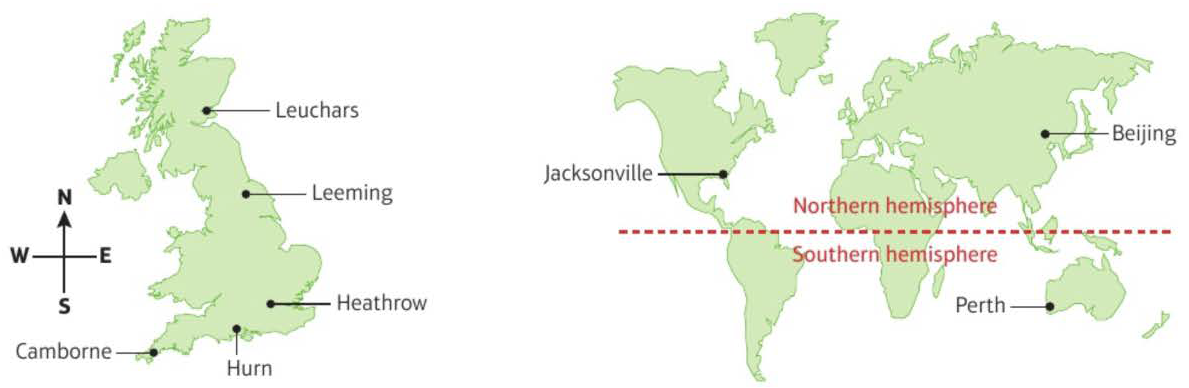
\includegraphics{LDSmap}\\
\begin{tabular}{|p{2cm}|p{15cm}|}
    \hline
    \textbf{City} & \textbf{Climate and geographical locations}                                                                                                           \\
    \hline
    Leuchars      & Coastal \newline NE of Scotland \newline Climate generally warm and temperate \newline significant rainfall throughout the year                       \\
    \hline
    Leeming       & \textbf{Inland} \newline Climate generally warm and temperate \newline significant rainfall throughout the year                                       \\
    \hline
    Heathrow      & \textbf{Inland} \newline Temperate oceanic climate \newline Cool to warm summers \newline cold winters                                                \\
    \hline
    Hurn          & Coastal \newline Southern England \newline Mild climate \newline Warm summers + \textbf{heavy rainfall} often in \textbf{mild} winters                \\
    \hline
    Camborne      & Coastal \newline Cornwall (SW England) \newline Climate generally warm and temperate \newline \textbf{High rainfall} even in driest months            \\
    \hline
    Beijing       & \textbf{Inland} (150km from the sea) \newline Northern hemisphere but relatively far South, so it tends to be \textbf{hot and humid} in summer months \\
    \hline
    Jacksonville  & Coastal \newline Northern hemisphere but relatively far South, so it tends to be \textbf{hot and humid} in summer months                              \\
    \hline
    Perth         & Coastal \newline In the \textbf{southern hemisphere} - in winter during May - Oct                                                                     \\
    \hline
\end{tabular}\\
(Cities are ordered from North to South)

%\subsection{Weather incidents}
\begin{description}
    \item[1987] ``Great storm" in UK in October so there are unusually high winds, mild ``El Nino" impact globally
    \item[2015] Strong ``El Nino" impact espacially in the US so there is cooler temperature and higher rainfall
\end{description}

\subsection{Data recorded}
%\subsection{Definitions}
\begin{tabular}{|p{5.5cm}|p{11.5cm}|}
    \hline
    \textbf{Variable}               & \textbf{Unit}                                                                                                                                                                                                      \\
    \hline
    Daily mean temperature          & The average of the hourly temperature (\textcelsius) readings, 09:00 – 09:00 GMT \newline A reading which is not available is listed as ‘n/a’.
    \\
    \hline
    Daily total rainfall            & Daily total precipitation (mm) 09:00 – 09:00 GMT
    (includes snow or hail, which is melted and measured in the same way as rainfall.) \newline
    'Trace' (tr) is less than 0.05 mm. \newline A reading which is not available will be shown by ‘n/a’
    \\
    \hline
    Daily total sunshine            & Sunshine amounts are recorded in hours and tenths and show the amount of bright sunshine recorded on the day of entry. \newline A reading which is not available will be shown by ‘n/a’                            \\
    \hline
    Daily maximum relative humidity & A measure of how close the air is to being saturated with water vapour. \newline Relative humidities above 95\% are associated with mist and fog. \newline A reading which is not available will be shown by ‘n/a’
    \\
    \hline
    Daily mean wind direction       & The daily mean wind direction the wind is \textbf{coming from}, (clockwise from North) is averaged and rounded to the nearest 10\textdegree \newline
    Readings which are not available are listed as ‘n/a’.
    \\
    \hline
    Daily mean windspeed            & Daily average windspeed \newline Readings are taken 00:00 – 00:00 GMT, in knots (kn, 1 knot = 1.15mph) \newline
    Readings which are not available are listed as ‘n/a’.                                                                                                                                                                                                \\
    \hline
    Daily maximum gust              & Maximum instantaneous wind speed \newline Readings are taken 00:00 – 00:00 GMT, in knots (kn, 1 knot = 1.15mph) \newline
    Readings which are not available are listed as ‘n/a’.                                                                                                                                                                                                \\
    \hline
    Daily maximum gust direction    & The direction from which the wind was blowing when the maximum gust during the hour commencing at the time of entry occurred, and is measured in degrees from true north.  \newline
    Readings which are not available are listed as ‘n/a’.                                                                                                                                                                                                \\
    \hline
    Daily mean cloud cover          & Measured in eights (oktas)                                                                                                                                                                                         \\
    \hline
    Daily mean visibility           & The greatest distance at which an object can be seen and recognized in daylight, or at night could be seen and recognized if the general illumination were raised to daylight level.
    \newline Visibility is measured horizontally, in decametres (Dm) dam = 10m \newline A dash (-) indicates data not available.
    \\
    \hline
    Daily mean pressure             & Mean sea level pressure, calculated from a measurement made at station level. \newline Measured in hectopascals (hPa) 	where 1 hPa = 1 millibar
    \\
    \hline
\end{tabular}
\subsection{Unit and precision of data}
\begin{tabular}{|l|l|l|}
    \hline
    \textbf{Variable}               & \textbf{Unit}               & \textbf{Precision}                           \\
    \hline
    Daily mean temperature          & \textcelsius                & to 1 dp                                      \\
    \hline
    Daily total rainfall            & mm                          & to 1 dp (tr = less than 0.05 mm, treat as 0) \\
    \hline
    Daily total sunshine            & hours                       & to 1 dp                                      \\
    \hline
    Daily maximum relative humidity & as a percentage             & nearest integer                              \\
    \hline
    Daily mean wind direction       & degree + cardinal direction & nearest integer                              \\
    \hline
    Daily mean windspeed            & knots / Beaufort conversion & nearest integer                              \\
    \hline
    Daily maximum gust              & knots                       & nearest integer                              \\
    \hline
    Daily maximum gust direction    & degree + cardinal direction & nearest integer                              \\
    \hline
    Daily mean cloud cover          & oktas                       & integer from 0-8                             \\
    \hline
    Daily mean visibility           & decametres (Dm)             & nearest 100                                  \\
    \hline
    Daily mean pressure             & hectopascals (hPa)          & nearest integer                              \\
    \hline
\end{tabular}
%* Wind direction is defined as the direction where the wind \textbf{comes from}

\subsection{Typical values}
\subsubsection{Temperature and wind speed}
\begin{tabular}{|l|l|l|}
    \hline
    \textbf{Location} & \textbf{Temperature range (\textcelsius)} & \textbf{Wind speed range (knots)} \\
    \hline
    Leuchars          & 4-19                                      & 3-23                              \\
    \hline
    Leeming           & 4-23                                      & 3-17                              \\
    \hline
    Heathrow          & 8-29                                      & 3-19                              \\
    \hline
    Hurn              & 6-24                                      & 2-19                              \\
    \hline
    Camborne          & 10-20                                     & 3-18                              \\
    \hline
    Beijing           & 8-33                                      & 2-9                               \\
    \hline
    Jacksonville      & 15-31                                     & 1-12                              \\
    \hline
    Perth             & 8-25                                      & 4-14                              \\
    \hline
\end{tabular}

\subsubsection{Other data}
\begin{tabular}{|p{4.8cm} | p{12.2cm}|}
    \hline
    \textbf{Variable}            & \textbf{Typical values}                                                  \\
    \hline
    Gust                         & 20 kn                                                                    \\
    \hline
    Rainfall                     & 0-60 mm in the UK, more extreme maximums elsewhere (e.g. 102mm in Perth) \\
    \hline
    Pressure                     & $1013 \pm 25$ Pa                                                         \\
    \hline
    Wind speed on Beaufort Scale & Mostly light / moderate. Maximum is fresh (5)                            \\
    \hline
    Sunshine                     & 0-16 hours                                                               \\
    \hline
    Cloud cover                  & 0-8 oktas                                                                \\
    \hline
\end{tabular}

\subsection{Cleaning data}
\begin{description}
    \item[tr] Needs to be replaced with a number between $0$ and $0.05$ (ideally $0.025$ as it is the midpoint) before processing data
    \item[n/a] Problem = data isn't available, usually ignored when doing calculations
\end{description}

\chapter{Measurements of location and spread}
\section{Types of means}
\begin{description}
    \item[Mean] $\overline{x}=\frac{\sum x}{n}$
    \item[Median] The middle value when the data values are put in order
    \item[Mode / modal class] The value or class that occurs most often
\end{description}

\section{Types of data}
\begin{description}
    \item[Quantitative data] Associated with numerical observations
    \item[Qualitative data] Associated with non-numerical observations
    \item[Continuous data] Can take any value in a given range
    \item[Discrete data] Can only take specific values in a given range
\end{description}

\section{Standard deviation / variance}
\begin{description}
    %\item $S_{xx}=\Sigma (x-\overline{x})^2=\Sigma x^2 - \frac{(\Sigma x)^2}{n}$
    \item[Variance] $\mathrm{Var}(x)=\frac{\Sigma x^2}{n} - (\frac{\Sigma x}{n})^2$
    \item[Standard deviation] $\sigma=\sqrt{\mathrm{Var}(x)}=\sqrt{\frac{\Sigma x^2}{n} - (\frac{\Sigma x}{n})^2}$
\end{description}

\section{Grouped data}
\subsection{Assumptions for estimating mean and standard deviation}
\begin{itemize}
    \item Values are evenly distributed within the classes
\end{itemize}

\section{Interpreting distributions}
\begin{description}
    \item[Measuring location] Mean / median / mode
    \item[Measuring spread of data] Variance / standard deviation / range / interpercentile ranges
\end{description}


\chapter{Representations of data}
\section{Outliers}
\begin{itemize}
    \item An extreme value that lies outside the overall pattern of data
    \item By default use $\text{LB} = \LQ - 1.5\times(\UQ-\LQ)$, $\text{UB} = \UQ + 1.5\times(\UQ-\LQ)$
\end{itemize}

\section{Cleaning data}
\begin{itemize}
    \item Anomalies (\textbf{not all outliers}) should be removed
    \item Anomalies = when the outlier is clearly an error and will be misleading
\end{itemize}


\section{Histogram}
\subsection{Reasons for using histograms}
\begin{itemize}
    \item Data is continuous
    \item Data is in groups (with uneven widths)
\end{itemize}
\subsection{Characteristics of histograms}
\begin{itemize}
    \item $\text{area}\propto\text{frequency}$
\end{itemize}

\section{Comparing data sets}
\begin{description}
    \item[Comparing location] A has a higher median / mean than B on average so A is ... than B on average
    \item[Comparing spread] A has a higher IQR / standard deviation than B so there is more variation in the \dots of A than B
\end{description}

\chapter{Correlation}
\section{Definitions}
\begin{description}
    \item[Bivariate data] Data which has pairs of related values
    \item[Independent / explanatory variable] The variable that the researcher can control, usually plotted on the x-axis
    \item[Dependent / response variable] The variable that the researcher measures, usually plotted on the y-axis
    \item[Correlation] Describes the nature of the linear relationship between 2 variables
\end{description}

\section{Causal relationships}
\begin{itemize}
    \item 2 variables have a casual relationship if a change in 1 variable causes a change in the other
    \item[$\star$] Correlation doesn't mean causation (add some explanations in context for questions)
\end{itemize}

\section{Linear regression}
* Work these out using a \textbf{calculator} in exams
\subsection{Regression equation for least squares regression line}
\begin{itemize}
    \item Regression line of $y$ on $x$: $y=a+bx$
    \item $b=\frac{\sum (x_i-\overline{x}) (y_i-\overline{y})}{\sum (x_i-\overline{x})^2}$ \textbf{(not needed for the exam)}
    \item $a=\overline{y}-b\overline{x}$
    \item Positive correlation: $b$ positive, negative correlation: $b$ negative
\end{itemize}

\subsection{Predicting values}
\begin{itemize}
    \item Should not extrapolate, only do interpolation
    \item Reliability: reliable as it is within the range of data / not reliable as it is extrapolating
    \item[$\star$] Not suitable for predicting $x$ based on $y$ (the independent variable in this model is $x$, you should not use this model to predict the value of $x$ based on $y$)
\end{itemize}

\subsection{Reason for using a regression line}
\begin{itemize}
    \item The data shows a strong (positive / negative) linear correlation
\end{itemize}


\chapter{Probability}
\section{Definitions}
\begin{description}
    \item[Experiment] A repeatable process that gives rise to a number of outcomes
    \item[Event] A set of one or more of these outcomes
    \item[Sample space] A set of all the possible outcomes
    \item[Mutually exclusive] Events cannot happen at the same time
    \item[Independent events] Whether one event happens does not affect the probability of the other happening
\end{description}



\chapter{Statistical distributions}
\section{Definitions}
\begin{description}
    \item[Random variable] One whose value depends on the outcome of a random event (outcome not known until the event took place)
    \item[Sample space] The range of values that the outcome can take
    \item[Discrete variable] Can only take certain numerical values
    \item[Probability distribution] Fully describes the probability of any outcome in the sample space
    \item[Uniform discrete distribution] All the probabilities are equal
\end{description}

\section{Notations}
\begin{itemize}
    \item Capital letters ($X$ or $Y$) denotes random variables
    \item Equivalent lowercase letters ($x$ or $y$) denotes particular values of the random variable
\end{itemize}

\subsection{Probability mass / density function}
\begin{itemize}
    \item $P(X=x) = \dots$ ($x=\dots$)
    \item You might need a large bracket e.g. \begin{math}
              P(X=x) = \begin{cases}
                  0.1 & x=1, 2                 \\
                  0.4 & x=3, 4                 \\
                  0   & x=\text{anything else}
              \end{cases}
          \end{math}
\end{itemize}

\section{Binomial distribution}
\subsection{Notation}
$X \sim B(n,p)$
\subsection{Probability calculation}
$\text{P}(x) = \dbinom{n}{x} p^x q^{n-x}$
\subsection{Assumptions}
\begin{itemize}
    \item There are a fixed number of trials, $n$
    \item There are two possible outcomes only (success and failure)
    \item There is a fixed probability of success, $p$
    \item The trials are independent of each other
\end{itemize}


\chapter{Hypothesis testing}
\section{Definitions}
\begin{description}
    \item[Hypothesis] A statement about the value of a population parameter
    \item[Test statistic] A value computer from sample data
    \item[Null hypothesis ($H_0$)] The hypothesis assumed to be correct ($\theta=\theta_0$)
    \item[Alternative hypothesis ($H_1$)] Tells you about the parameter if $H_0$ is rejected as a result of the test ($\theta \neq \theta_0$ / $\theta>\theta_0$ (right tail) / $\theta<\theta_0$ (left tail))
    \item[Significance level ($\alpha$)] Probability of rejecting $H_0$ when assuming $H_0$ is true
    \item[Critical region] A region of the probability distribution which, if the test statistic falls within it, would cause you to reject the null hypothesis
    \item[Critical value] The first value to fall inside the critical region / a value that is compared to the test statistic to determine whether to reject $H_0$
    \item[Acceptance region] The rejection region for $H_1$ in the testing of a hypothesis
    \item[Actual significance level] The probability of incorrectly rejecting the null hypothesis (when $H_0$ is actually true)
\end{description}

\section{Test on proportion / probability of success assuming binomial distribution}
$t^*$ = test statistics
\subsection{By critical value}
\begin{itemize}
    \item One tailed: if stats test $t^* > \text{cv}$ or $t^* < \text{cv}$ (depends on right / left tail): reject $H_0$, else accept $H_0$
    \item Two tailed: if stats test $t^* > \text{upper cv}$ or $t^* < \text{lower cv}$: reject $H_0$, else accept $H_0$ (For 2 tailed tests the probability used for calculating cv at the end of each tail = $\frac{\alpha}{2}$)
\end{itemize}


\subsection{By $p$ value}
\begin{itemize}
    \item One tailed: if $P(t\geq t^*) < \alpha$: reject $H_0$, else accept $H_0$
    \item Two tailed: if $P(t\geq t^*) < \frac{\alpha}{2}$ or $P(t\leq t^*) > \frac{\alpha}{2}$: reject $H_0$, else accept $H_0$
\end{itemize}

\begin{comment}
\subsection{Presenting the solution}
\begin{enumerate}
    \item Define the test statistic, $X$ and the parameter, $p$
    \item Formulate a model for $X$ ($X \sim B(n, p)$)
    \item Write down $H_0$ and $H_1$ as statements involving $p$ (these determine whether your test is one or two-tailed)
    \item Specify the significance level
    \item Decide whether to reject $H_0$ by comparing $t^*$ to critical value or finding the probability of $t^*$ taking $x$ or a more extreme value
    \item State your conclusion: there is / is not sufficient evidence to reject $H_0$ + a statement \textbf{in the context of the question}
\end{enumerate}

\end{comment}


\section{Two tailed tests}
\begin{itemize}
    \item Halve the significance value to find out the critical region at each end unless otherwise specified
    \item Notice if the question asks for the probability in each tail to be \textbf{as close to $\frac{\alpha}{2}$ as possible}
    \item Always use 2 tailed tests if whether testing for increase / decrease in $p$ is not specified
\end{itemize}

\section{Example responses}
\subsection{One tailed + critical region}
\begin{example}
    A single observation is taken from $X\sim B(10, p)$ and $x=1$ is obtained. Use this value to test $H_0: p=0.4$ against $H_1:p<0.4$ using a $5\%$ significance level
\end{example}

\begin{solution}
    $H_0: p=0.4$\\
    $H_1:p<0.4$\\
    Test statistic: $x=1$\\
    $\text{Significance level} = 5\%$\\
    One-tailed test\\
    $P(X \leq c_1) < 0.05$\\
    $P(X \leq 1) = 0.0463$ ($P(X \leq 2) = 0.1672$ too big)\\
    $c_1 = 1$ so critical region is $X\leq 1$\\
    $x=1$ lies in the critical region, so evidence suggests rejecting $H_0$ at $5\%$ significance level
\end{solution}

\subsection{One tailed + $p$ value}
\begin{example}
    A single observation is taken from $X\sim B(10, p)$ and $x=5$ is obtained. Use this value to test $H_0: p=0.25$ against $H_1:p>0.25$ using a $5\%$ significance level
\end{example}

\begin{solution}
    $H_0: p=0.25$\\
    $H_1:p>0.25$\\
    Test statistic: $x=5$\\
    $\text{Significance level} = 5\%$\\
    One-tailed test
    \begin{align*}
        P(X\geq 5) & = 1-P(X\leq 4) \\ &= 0.0781
    \end{align*}
    Compare $p$-value with significance level: $0.0781 > 0.05$\\
    It is not significant so no evidence to reject $H_0$ at the 5\% significance level
\end{solution}

\subsection{Two tailed - find critical region when using `probability as close to'}
\begin{example}
    $Y \sim B(25, p)$, given that $H_0: p=0.42$, $H_1:p \neq 0.42$, find the critical region for the test using $10\%$ significance level, \textbf{the probability in each tail should be as close to $5\%$ as possible}
\end{example}

\begin{solution}
    $P(Y\leq c_1)$ as close to 0.05 as possible\\
    $P(Y\leq 6) = 0.0495 < 0.05$ - closest to $0.05$ so $c_1 = 6$\\
    $P(Y\leq 7) = 0.1106 > 0.05$\\\\

    $P(Y\geq c_2)$ as close to 0.05 as possible $\rightarrow$ $1-P(Y\leq c_2 -1)$ as close to 0.05 as possible $\rightarrow$ $P(Y\leq c_2 -1)$ as close to 0.95 as possible\\
    $P(Y\leq 14) = 0.9465 < 0.95$ - closest to $0.05$ so $c_2 = 14+1 = 15$\\
    $P(Y\leq 15) = 0.19779 > 0.95$
\end{solution}


\part{Applied 1 Mechanics}
\setcounter{chapter}{7}
\chapter{Modelling in mechanics}
\section{Modelling assumptions}
\begin{tabular}{|m{3.9cm} | m{13.5cm}|}
    \hline
    \textbf{Model}            & \textbf{Assumptions}                                                                                                                                                                                    \\
    \hline
    Particle                  & Mass of the object is concentrated at a single point, rotational effect of external forces and air resistance can be ignored, volume is negligible                                                      \\
    \hline
    Rod                       & Mass is concentrated along a line, no thickness, rigid                                                                                                                                                  \\
    \hline
    Lamina                    & Mass is distributed across a flat surface                                                                                                                                                               \\
    \hline
    Uniform body              & Mass is concentrated at the centre of mass                                                                                                                                                              \\
    \hline
    Light object              & Treat the object as if it has zero mass, tension is the same at both ends of the string                                                                                                                 \\
    \hline
    Inextensible string / rod & Tension / thrust is the same at any point on the string / rod, any stretching effect can be ignored, \textbf{same acceleration and velocity throughout the system}                                      \\
    \hline
    Smooth surface            & No friction between the surface and other objects                                                                                                                                                       \\
    \hline
    Rough surface             & Objects experience a frictional force if they are moving or acted on by a force                                                                                                                         \\
    \hline
    Wire                      & Treat as one-dimensional, doesn't bend (rigid)                                                                                                                                                          \\
    \hline
    Smooth and light pulley   & Pulley has no mass, tension is the same on either side of the pulley, no friction around the pulley                                                                                                     \\
    \hline
    Bead                      & Mores freely along a wire or string, tension is the same on either side                                                                                                                                 \\
    \hline
    Peg                       & Dimensionless and fixed, can be rough or smooth                                                                                                                                                         \\
    \hline
    Air resistance            & Usually negligible                                                                                                                                                                                      \\
    \hline
    Gravity                   & All objects with mass are attracted towards the Earth, gravity is uniform and acts vertically downwards, $g$ is constant and is taken as $9.8 \: \mathrm{m} \: \mathrm{s}^{-2}$ unless otherwise stated \\
    \hline
\end{tabular}

\chapter{Constant acceleration}
\section{SUVAT equations}
\begin{itemize}
    \item $s=ut+\frac{1}{2}at^2$
    \item $s=vt-\frac{1}{2}at^2$
    \item $v=u+at$
    \item $v^2=u^2+2as$
    \item $s=\frac{1}{2}(u+v)t$
\end{itemize}

\section{$v$-$t$ graphs}
\subsection{Limitations of the graph}
\begin{itemize}
    \item Instantaneous change in acceleration is unrealistic
    \item Unlikely to remain at constant acceleration
\end{itemize}

\chapter{Forces and motion}
\section{Types of forces}
\begin{description}
    \item[Weight:] $W=mg$
    \item[Normal contact force:] symbol = $R$ or $N$
    \item[Static friction:] Depends on driving force, $F\leq \mu R$
    \item[Dynamic friction:] $f=\mu R$ ($\mu$=coefficient of kinetic friction), exists on \textbf{rough surfaces}
    \item[Thrust / compression:] Object being pushed along using a light rod
    \item[Tension:] $T=\text{elastic coefficient}\times\text{extension}=k\times\Delta x$
    \item[Air resistance / drag:] resistance due to air / water / fluid
    \item[Driving / propulsive force:] forward force produced by the object itself
\end{description}

\section{Common scenarios}
\subsection{Connected particles}
\begin{itemize}
    \item Acceleration is the same across the whole system
    \item Internal force can be ignored
    \item Tension at the same rope has the same magnitude
\end{itemize}

\subsection{Lift}
\begin{itemize}
    \item Consider the whole system to find tension in the string
    \item Consider one object only to find force they exerted on each other
    \item Rising: $R-W=ma$
    \item Moving down: $W-R=ma$
    \item On rest: $R=W$
\end{itemize}

\subsection{Fixed pulley}
\begin{itemize}
    \item Same tension
    \item Same magnitude for acceleration (different direction)
    \item Use simultaneous equations to find tension
    \item $\text{Force on pulley} = 2 \times \text{tension}$
\end{itemize}

\chapter{Variable acceleration}
\section{Finding distance travelled}
\begin{itemize}
    \item Use graph to show sign changes during the interval
    \item Remember to account for periods with negative velocity
\end{itemize}


\part{Applied 2 Statistics}
\setcounter{chapter}{0}
\chapter{Regression, correlation and hypothesis testing}

\section{PMCC}
\begin{itemize}
    \item Measures the strength of \textbf{linear} correlation
    \item $r =\frac{\sum\left(x_{i}-\bar{x}\right)\left(y_{i}-\bar{y}\right)}{\sqrt{\sum\left(x_{i}-\bar{x}\right)^{2} \sum\left(y_{i}-\bar{y}\right)^{2}}}$ \textbf{(not needed for the exam)}
\end{itemize}

\section{Converting to linear form}
\subsection{Commenting on appropriateness}
\begin{itemize}
    \item \dots gives a linear relationship between \dots
    \item PMCC is close to $1$ or $-1$ which supports the use of a linear model
\end{itemize}

\section{Hypothesis test for zero linear correlation}
\subsection{Template}
\begin{itemize}
    \item $H_0$: $\rho = 0$
    \item $H_1$: $\rho \neq 0$ (two tailed) / $\rho > 0$ (right tail) / $\rho < 0$ (left tail)
    \item Sample size = $\dots$
    \item Significance level = $\dots$
    \item The critical value of $r$ for this test is $\dots$
    \item The observed value of $r$ is $\dots$
    \item $\dots < \dots$ so the observed value of $r$ is inside / outside the critical region
    \item So reject / accept $H_0$
    \item Conclusion
\end{itemize}




%\subsection{Sample variance}
%\begin{itemize}
%	\item $S^2=\frac{\Sigma(x_i-\overline{x})^2}{n-1}=\frac{1}{n-1}(\Sigma x_i^2-\overline{x}^2n)=\frac{1}{n-1}(\Sigma x_i^2-\frac{(\Sigma x)^2}{n})$
%\end{itemize}

\chapter{Conditional probability}
\section{Conditional probability formula}
\begin{itemize}
    \item $P(A|B) = \frac{P(A \cap B)}{P(B)}$
\end{itemize}
\section{Principle of inclusion-exclusion}
\begin{itemize}
    \item $P(A\cup B)=P(A)+P(B)-P(A\cap B)$
\end{itemize}

\chapter{The normal distribution}
\section{Notation}
\begin{itemize}
    \item $X \sim N(\mu,\sigma^2)$
    \item $\mu$ = mean of the population
    \item $\sigma^2$ = \textbf{variance} of the data
\end{itemize}
\section{Properties}
\begin{itemize}
    \item The data is \textbf{continuous}
    \item Has parameters $\mu$ (mean) and $\sigma^2$ (variance)
    \item Is symmetrical: mean = median = mode
    \item Has a bell-shaped curve with asymptotes at each end
    \item Total area under the curve = $1$
    \item Has points of inflection at $\mu+\sigma$ and $\mu-\sigma$
\end{itemize}

\section{Estimating probabilities}
\begin{itemize}
    \item $68\%$ of observations lie within $\pm 1$ standard deviation of the mean
    \item $95\%$ of observations lie within $\pm 2$ standard deviation of the mean
    \item $99.8\%$ of observations lie within $\pm 3$ standard deviation of the mean
\end{itemize}
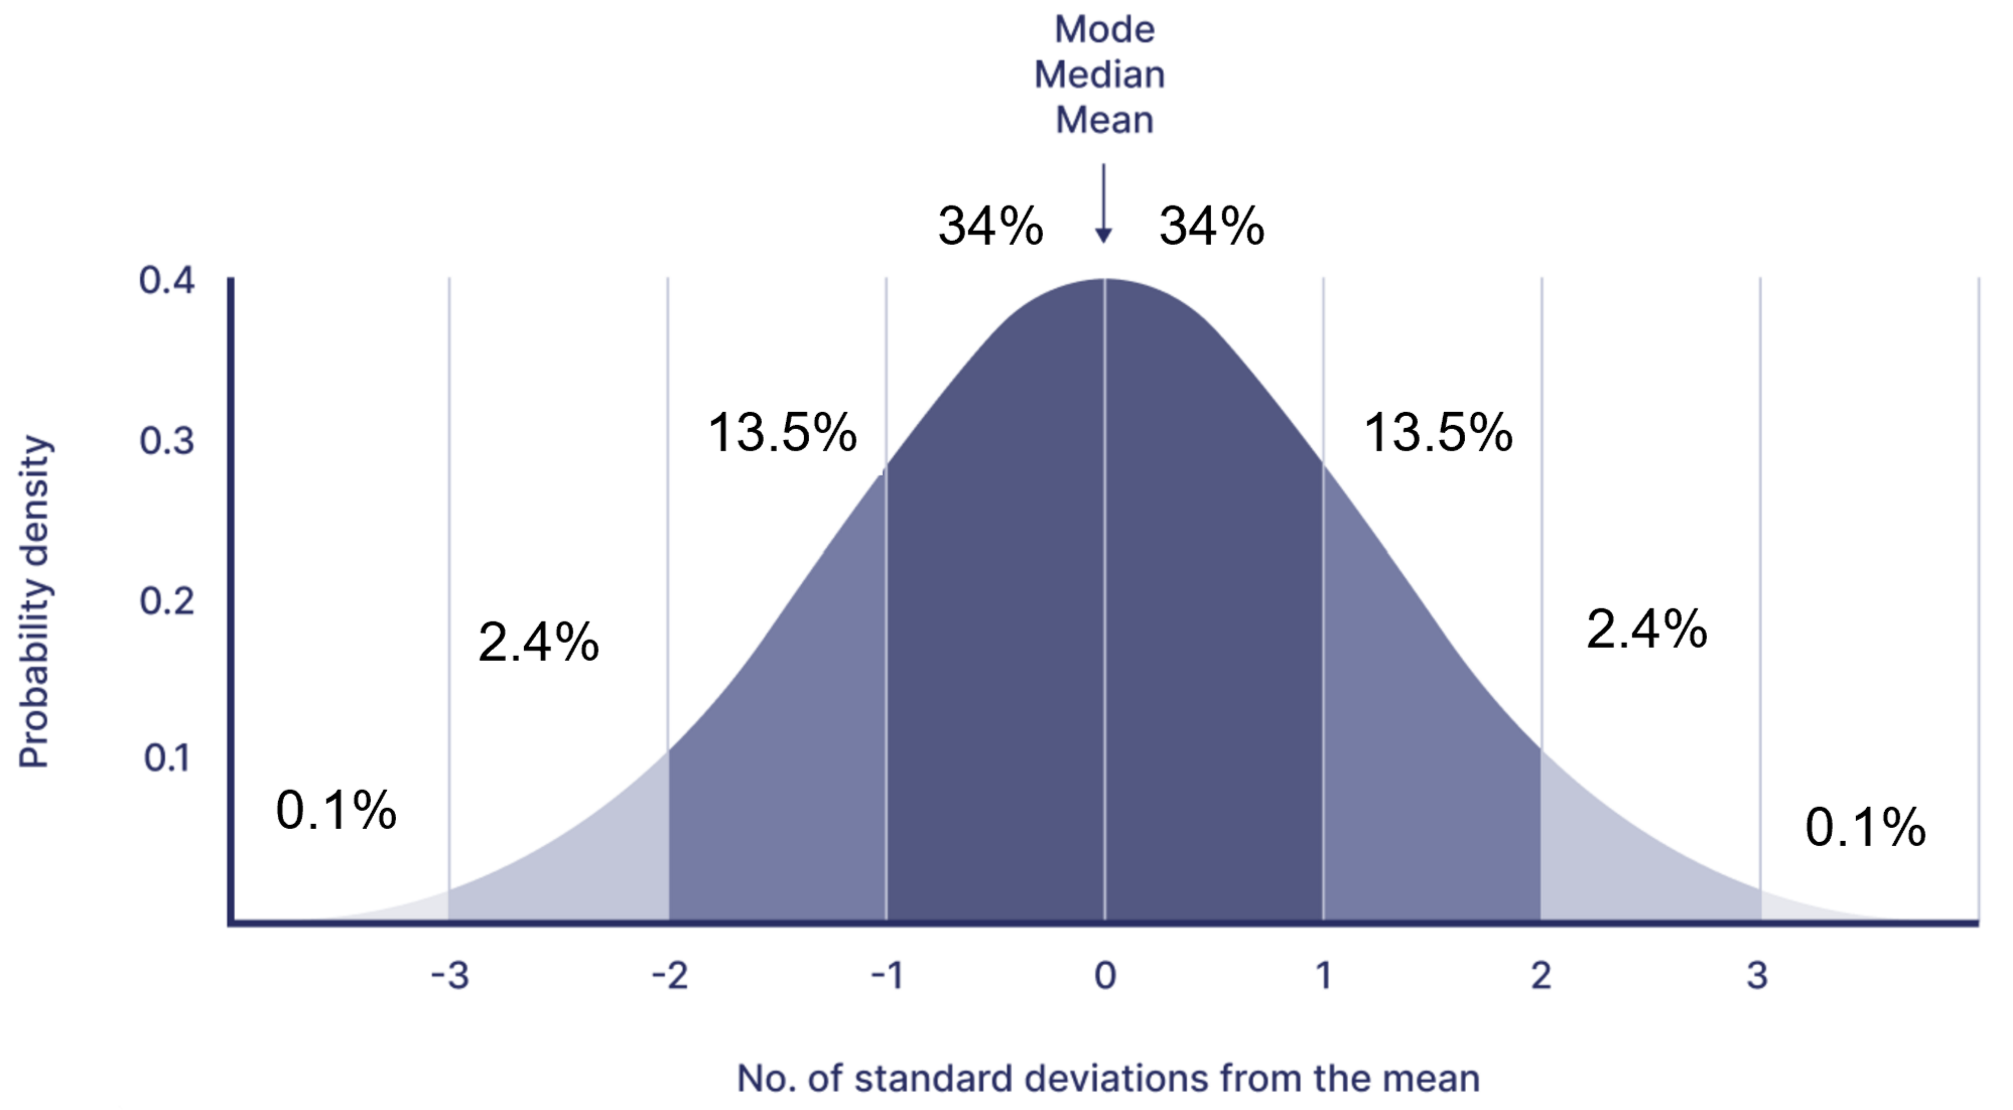
\includegraphics[width=0.7\linewidth]{images/normal_estimate}

\section{Approximation of binomial distribution}
If $n$ is large ($n\geq35$) and $p$ is close to $0.5$, then $X \sim B(n,p)$ can be modelled as $$Y \sim N(np, np(1-p))$$
\subsection{Approximations}
\begin{itemize}
    \item $\text{P}(X\geq a)\approx \text{P}(Y\geq [a-0.5])$
    \item $\text{P}(X=a)\approx \text{P}([a-0.5]<Y<[a+0.5])$
    \item $\text{P}(X \leq a)\approx \text{P}(Y\leq [a+0.5])$
\end{itemize}


\section{Sample mean}
If $n$ is large enough ($n\geq35$) and $X\sim N(\mu, \sigma^2)$, then sample mean $\overline{X}$ is
normally distributed:
$$\overline{X} \sim N\left(\mu, \frac{\sigma^2}{n}\right)$$


\part{Applied 2 Mechanics}
\setcounter{chapter}{3}
\chapter{Moments}
\section{Definition}
\textbf{Turning} effect of the force on a rigid body.\\
Clockwise moment of $F$ about P: $|F|\times d= \vec{F}\times\vec{d} = |F||d|\sin\theta$
\section{Tilting about a pivot}
Support / tension force at any point = 0\\
Show $\text{moment} \neq 0$

\chapter{Forces and friction}
\section{Resolving forces}
\begin{enumerate}
    \item Resolve perpendicular and parallel to the direction of motion
    \item Clearly indicate the direction of motion
    \item Use $\sum F = ma$
\end{enumerate}

\section{Friction}
\begin{itemize}
    \item $F_r \leq \mu R$
    \item Friction is only \textbf{as large as it needs to be} to oppose the motion
    \item If the object is moving then $F_r = \mu R$
\end{itemize}



\chapter{Projectiles}
\section{Assumptions}
\subsection{Modelling as particle}
\begin{itemize}
    \item All of the weight act at one point (specify the point)
    \item Air resistance can be ignored
    \item Any rotational forces can be ignored
\end{itemize}

\section{Equation of projectiles}
\begin{description}
    \item[Time of flight (back to the released height)] $T=\frac{2U\sin\alpha}{g}$
    \item[Time to reach the greatest height] $\frac{U\sin\alpha}{g}$
    \item[Range on horizontal plane] $\frac{U^2\sin 2\alpha}{g}$
    \item[Greatest height reached] $\frac{U^2\sin^2\alpha}{2g}$
    \item[Equation of trajectory] $y=x\tan\alpha - gx^{2}\frac{\left(1+\tan^2\alpha\right)}{2U^2}$ 
\end{description}

\section{Model limitations}
\begin{itemize}
    \item Approximate value of $g$ have been used
    \item Dimensions of the stone can affect its motion
    \item $g$ has been assumed to be constant
    \item Effect of wind is ignored
    \item Spin of the stone ignored
    \item Surface area of the ball ignored / dimensions of the ball ignored / ball modelled as particle
    \item Air resistance ignored
\end{itemize}

\chapter{Applications of forces}
\section{Pulleys on slope}
\subsection{Force on pulley}
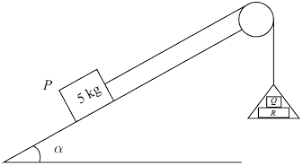
\includegraphics[width = 0.4\linewidth]{pulley_slope.png}
\begin{itemize}
    \item $F=2T\cos\left(\frac{90-\alpha}{2}\right)$
    \item Note that we need to consider the \textbf{direction} of the force
\end{itemize}

\chapter{Further kinematics}
\section{Hyperbolic function definitions}
\subsection{$\sinh x$}
\begin{description}
	\item[Definition] $\sinh x = \dfrac{e^x-e^{-x}}{2}$
	\item[Domain] $x \in \textbf{R}$
	\item[Asymptotes] $x\rightarrow +\infty$, $y\rightarrow\dfrac{e^x}{2}$; $x\rightarrow -\infty$, $y\rightarrow -\dfrac{e^{-x}}{2}$
	\item[x-intercept] $(0,0)$
	\item[y-intercept] $(0,0)$
	\item[Graph]
\end{description}

\subsection{$\cosh x$}
\begin{description}
	\item[Definition] $\cosh x = \dfrac{e^x+e^{-x}}{2}$
	\item[Domain] $x \in \textbf{R}$
	\item[Asymptotes] $x\rightarrow +\infty$, $y\rightarrow\dfrac{e^x}{2}$; $x\rightarrow -\infty$, $y\rightarrow\dfrac{e^{-x}}{2}$
	\item[x-intercept] No
	\item[y-intercept] $(0,1)$
	\item[Graph]
\end{description}

\subsection{$\tanh x$}
\begin{description}
	\item[Definition] $\tanh x = \dfrac{\sinh x}{\cosh x}=\dfrac{e^x-e^{-x}}{e^x+e^{-x}}$
	\item[Domain] $x \in \textbf{R}$
	\item[Asymptotes] $x\rightarrow +\infty$, $y\rightarrow 1$; $x\rightarrow -\infty$, $y\rightarrow -1$
	\item[x-intercept] $(0,0)$
	\item[y-intercept] $(0,0)$
	\item[Graph]
\end{description}

\subsection{$\csch x$}
\begin{description}
	\item[Definition] $\csch x = \dfrac{1}{\sinh x}$
	\item[Domain] 
	\item[Asymptotes] 
	\item[x-intercept] 
	\item[y-intercept] 
	\item[Graph]
\end{description}


\subsection{$\sech x$}
\begin{description}
	\item[Definition] $\sech x = \dfrac{1}{\cosh x}$
	\item[Domain] 
	\item[Asymptotes] 
	\item[x-intercept] 
	\item[y-intercept] 
	\item[Graph]
\end{description}


\subsection{$\coth x$}
\begin{description}
	\item[Definition] $\coth x = \dfrac{\cosh x}{\sinh x}$
	\item[Domain] 
	\item[Asymptotes] 
	\item[x-intercept] 
	\item[y-intercept] 
	\item[Graph]
\end{description}

\section{Identities of hyperbolic functions}
Similar to trigonometric identities:
\begin{itemize}
	\item $\tanh x = \dfrac{\sinh x}{\cosh x}$
	\item $\cosh^2 x - \sinh^2 x = 1$
	\item $\tanh^2 x + \sech^2 x= 1$
	\item $\coth^2 x - \csch^2 x = 1$
\end{itemize}

\subsection{Addition}
\begin{itemize}
	\item $\sinh(x+y)=\sinh x \cosh y + \sinh y \cosh x$
	\item $\cosh(x+y)=\cosh x \cosh y + \sinh x \sinh y$
	\item $\tanh(x+y) = \dfrac{\sinh(x+y)}{\cosh(x+y)} = \dfrac{\sinh x \cosh y + \sinh y \cosh x}{\cosh x \cosh y + \sinh x \sinh y} = \dfrac{\frac{\sinh x}{\cosh x}+\frac{\sinh y}{\cosh y}}{1 + \frac{\sinh x \sinh y}{\cosh x \cosh y}}=\dfrac{\tanh x + \tanh y}{1 + \tanh x \tanh y}$
\end{itemize}

\subsection{Double angle}
\begin{itemize}
	\item $\sinh 2x = 2\sinh x \cosh x$
	\item $\cosh 2x = \cosh^2 x + \sinh^2 x = 2\cosh^2 x - 1 = 2\sinh^2 + 1$
	\item $\tanh 2x = \dfrac{2\tanh x}{1 + \tanh^2 x}$
\end{itemize}

\subsection{Power descending}


\section{Differentiating hyperbolic functions}
\begin{itemize}
	\item $(\sinh x)'=\cosh x$
	\item $(\cosh x)'=\sinh x$
	\item $(\tanh x)'=1-\tanh^2 x = \sech^2 x$
	\item $(\csch x)'=-\coth x \csch x$
	\item $(\sech x)'=-\sech x \tanh x$
	\item $(\coth x)'=-\sech^2 x$
\end{itemize}


\end{document}